\documentclass[a4paper,10pt]{article}
\usepackage[margin=2.5cm]{geometry}
\usepackage[utf8]{inputenc}
\usepackage[colorlinks=true,urlcolor=blue]{hyperref}
\usepackage{amsmath}
\usepackage{graphicx}
\usepackage{float}
\usepackage{caption}

%\usepackage{listings} %Alternative to minted
\usepackage{minted}



\setlength{\parindent}{0em}
\setlength{\parskip}{1em}

\title{\textbf{Deep Learning for Image Analysis} 
\\ DL4IA -- Report for Assignment X}
\author{Student Y}
\date{\today}

\begin{document}

\maketitle

\section{Introduction}

This document can be used as an assignment report template. 

Always indicate the question number associated with your answer (e.g., ``Exercise 1.4.2'' for the second sub-task of Exercise 1.4). To make your report readable as a stand alone document, 
please either include a brief repetition of the assignment questions, or answer such that it is clear what is addressed in your text and the context of your statements and observations given (i.e., do not just answer ``42'', but instead write out ``The answer to the Ultimate Question of Life, the Universe, and Everything is 42.''\cite{Adams}). 
Make sure that every figure, table, and code has a caption and is referenced to in your text. Do not forget to put your name into the report.

When writing code, make isolated functions for the specific parts of your code. This will make it easier to include it in your report but, more importantly, will help you to structure your code. You do not need to include the full code in the report but are asked to include important parts to show that you have solved the problem in a correct way. Remember if you have a function that calls another function you need to include both of them or write what the other function does and returns. Always \textbf{attach the complete code} (possibly as a zip archive) together with the report.

\section{Mathematical exercises}

To present mathematical derivations and expression you should write the derivations directly in \LaTeX\ 

\textbf{\LaTeX\ example:}

Given the linear regression model:
\begin{equation}
    z_i = \sum_{j=1}^p w_jx_{ij} 
\end{equation}

with the cost function 
\begin{equation}
\label{eq:cost}
\begin{split}
    J = \frac{1}{n}\sum_{i=1}^nL_i \\
    \text{where } L_i = (y_i-z_i)^2    
\end{split}
\end{equation}


\textit{\textbf{Exercise 1.}}
\begin{equation*}
    \frac{\delta J}{\delta w} = ...
\end{equation*}

\begin{equation*}
    \frac{\delta J}{\delta b} = ...
\end{equation*}


\textit{\textbf{Exercise 2.}}

\begin{equation*}
\begin{split}
    \frac{\delta J}{\delta z_i} = ... \\
    \vdots
\end{split}
\end{equation*}


\section{Code exercises}

For exercises where you are asked to write code, include the important functions and steps that you have implemented. For functions it is good practise to always have a small description in the beginning of the function, explaining what the function does, what the arguments are and what is returned. In \LaTeX\ you can for instance use the \emph{minted} package to include code 
%(read more about listings \href{https://www.overleaf.com/learn/latex/code_listing}{here}).
(read more about minted \href{https://www.overleaf.com/learn/latex/Code_Highlighting_with_minted}{here}).


\hfill \break
\textit{\textbf{Exercise 3.} Implement a gradient descent algorithm ...}

Based on the derivations given in exercise 1 and 2, the following functions are implemented to perform gradient descent for linear regression. 

\begin{itemize}
\item
The \emph{initialize} function is used to initialize the weights and offsets by method X.
\item
The \emph{cost} function takes \ldots and \ldots as input and calculates the cost according to eq. \eqref{eq:cost}.
\end{itemize}

\begin{minted}[frame=lines,framesep=2mm,linenos]{python}

def initialize(arg1, arg2, ...):
    """ param arg1: description of argument 1
        param arg2: description of argument 2
        ...
        
        return: description of what the function returns
    """
    
    w = ...
    b = ...
    
    
    return w, b

def cost(arg1, arg2, ...):
    """ param arg1: description of argument 1
        param arg2: description of argument 2
        ...
        
        return: description of what the function returns
    """
    
    J = 
    
    return J

\end{minted}

\newpage
\hfill \break
The weights and offsets are optimized to minimize the cost as follows:

\begin{minted}[frame=lines,framesep=2mm,linenos]{python}

w,b = initialize(*args) #Initialize weights and offsets
n_iterations = 1000 #Number of gradient descent iterations

for it in range(n_iterations):
    
    ...
    
    J = cost(*args)
\end{minted}


\section{Results}
When presenting results, include plots of the optimization process, quantitative scores for your models and other relevant stuff to show the performance of your models. An easy to use and well documented library in python is \emph{Matplotlib} (\href{https://matplotlib.org/}{link}). 
For plots, \textbf{always} write a caption explaining what is shown in the plot, and also what can be observed/concluded from the plot. Remember to always have labels on the axes, and when suitable a legend (if multiple plots in same figure). Make the plots of a suitable size to be visible (if printed). See Figure \ref{fig:cost_per_iteration} for an example.


\begin{figure}[H]
 \centering
    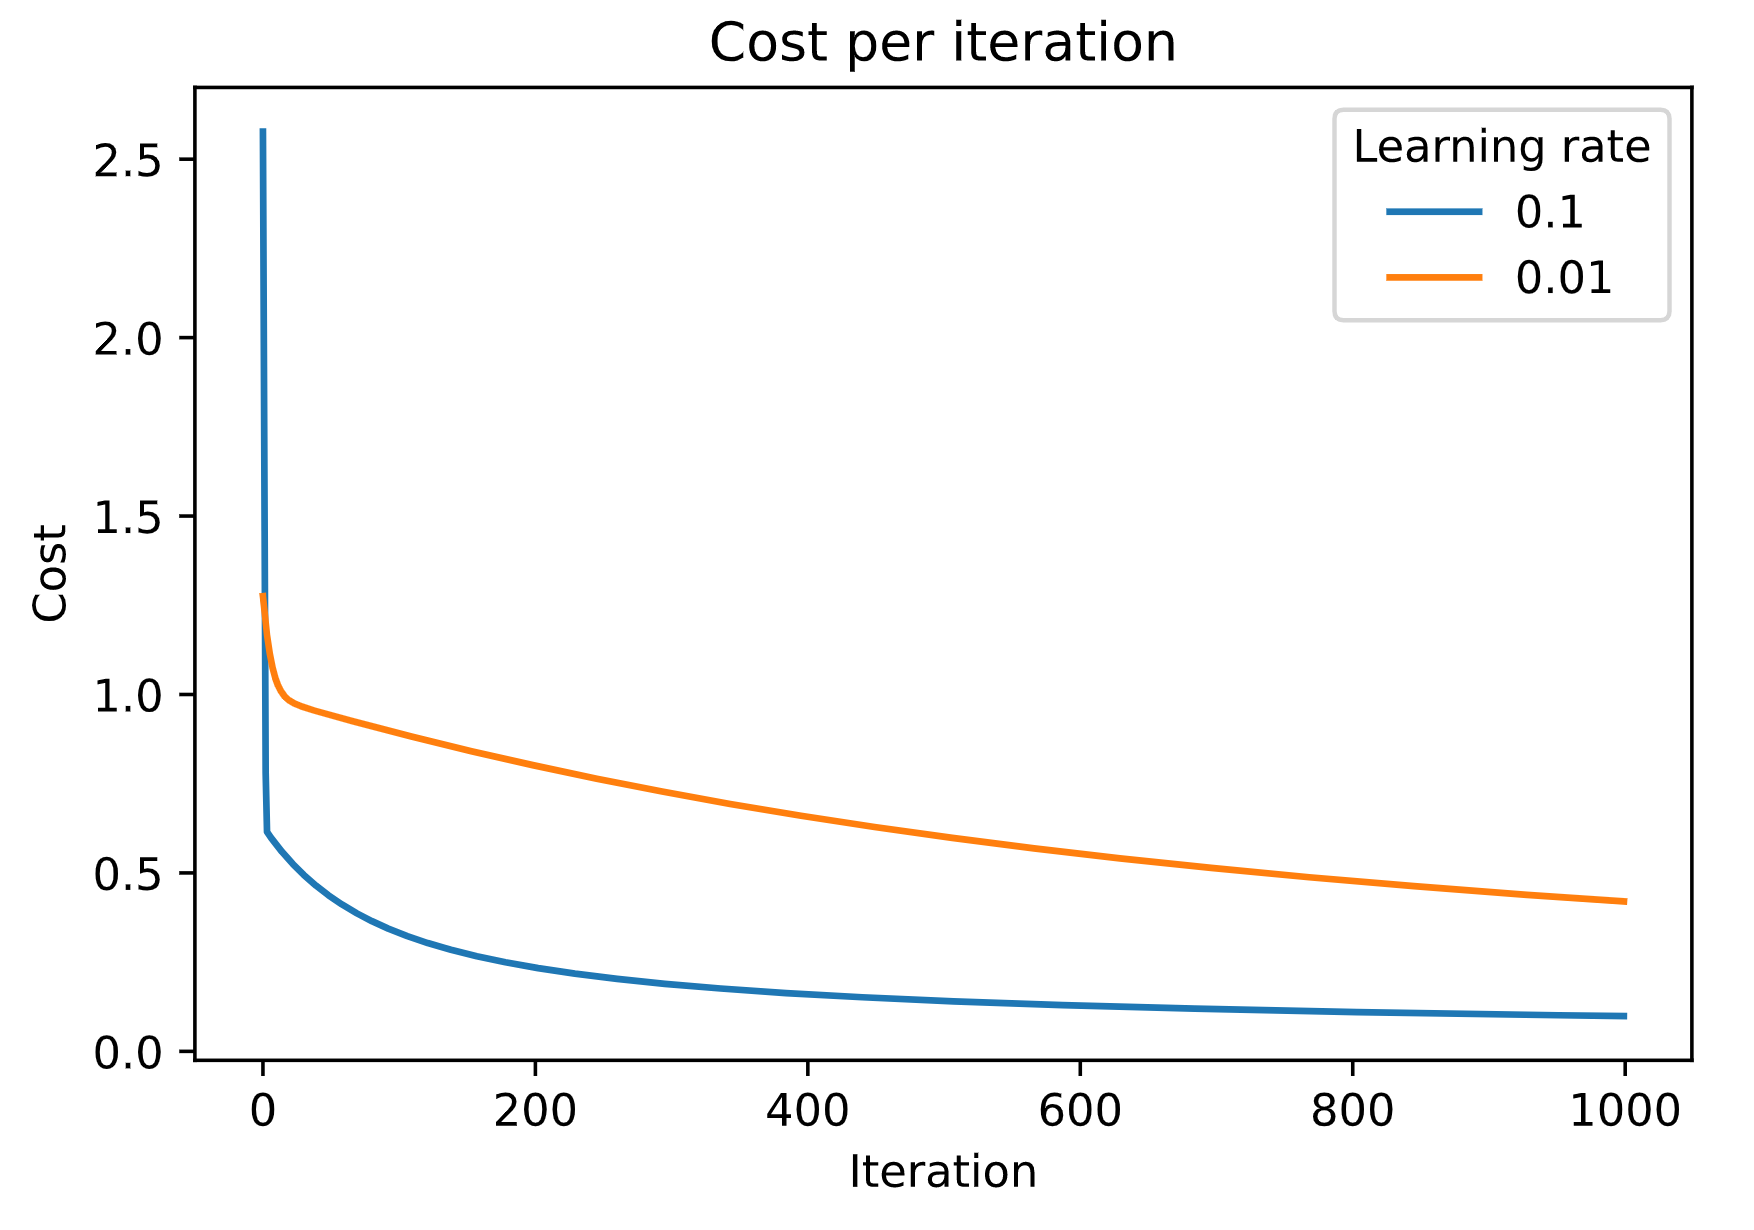
\includegraphics[width=0.6\textwidth]{cost_per_iteration_lr.png}
    \caption{Plot showing how the cost \eqref{eq:cost}, evaluated on the training sets, is changing with with number of iterations. It can be seen that\ldots}
    \label{fig:cost_per_iteration}
\end{figure}



\begin{thebibliography}{1}

\bibitem{Adams} Adams, Douglas (1979). The Hitchhiker's Guide to the Galaxy. Pocket Books. p. 3.

\end{thebibliography}

\end{document}
